\documentclass[11.5pt]{sig-alternate} % sets document style to sig-alternate
% packages
% typesetting
%\usepackage{dirtytalk} % typset quotations easier (\say{stuff})
\usepackage{hanging} % hanging paragraphs
\usepackage[defaultlines=3,all]{nowidow} % avoid widows
\usepackage[pdfpagelabels=false]{hyperref} % produce hypertext links, includes backref and nameref
\usepackage{xurl} % defines url linebreaks, loads url package
\usepackage{microtype}
\usepackage{textgreek}
%\usepackage{textcomp}
%\newcommand{\texttildemid}{\raisebox{0.4ex}{\texttildelow}}
% layout
\usepackage{enumitem} % control layout of itemize, enumerate, description
\usepackage{fancyhdr} % control page headers and footers
\usepackage{float} % improved interface for floating objects
%\usepackage{multicol} % intermix single and multiple column pages
% language
\usepackage[utf8]{inputenc} % accept different input encodings
\usepackage[english]{babel} % multilanguage support
% misc
\usepackage{graphicx} % builds upon graphics package, \includegraphics
%\usepackage{lastpage} % reference number of pages
%\usepackage{comment} % exclude portions of text (?)
\usepackage{xcolor} % color extensions
\usepackage[backend=biber, style=apa]{biblatex} % sophisticated bibliographies % necessary for HTML to display author info and date on abstract page
\usepackage{csquotes} % advanced quotations, makes biblatex happy
\usepackage{authblk} % support for footnote style author/affiliation
% tables and figures
\usepackage{tabularray}
%\usepackage{array} % extend array and tabular environments
\usepackage{caption} % customize captions in figures and tables (rotating captions, sideways captions, etc)
%\usepackage{cuted} % allow mixing of \onecolumn and \twocolumn on same page
\usepackage{multirow} % create tabular cells spanning multiple rows
%\usepackage{subfigure} % deprecated, support for manipulation of small figures
%\usepackage{tabularx} % extension of tabular with column designator "x", creates paragraph-like column whose width automatically expands
%\usepackage{wrapfig} % allows figures or tables to have text wrapped around them
%\usepackage{booktabs} % better rules
% dummy text
%\usepackage{blindtext} % blind text dummy text
%\usepackage{kantlipsum} % Kant style dummy text
\usepackage{lipsum} %lorem ipsum dummy text
% other helpful packages may be booktabs, longtable, longtabu, microtype

\pagestyle{fancy} % sets pagestyle to fancy for fancy headers and footers

% header and footer
% modern way to set header image
\renewcommand{\headrulewidth}{0pt} % defines thickness of line under header
\renewcommand{\footrulewidth}{0pt} % defines thickness of line above header
\setlength\headheight{80.0pt} % sets height between top margin and header image, effectively moves page contents down
\addtolength{\textheight}{-80.0pt} % seems to affect the lower height. maybe only works properly if footer numbers enabled?
\fancyhf{}
\fancyhead[CE, CO]{
\includegraphics[width=\textwidth]{headerImage.png}}
% footer
%\fancyfoot[LE,LO]{Article Title Here \\ DOI: }% left footer article title and doi
%\fancyfoot[CE,CO]{{}} % center footer empty
%\fancyfoot[RE,RO]{\thepage} % right footer page numbers
%\pagenumbering{arabic} % arabic (1, 2, 3) numbering in footer

\hypersetup{colorlinks=true,urlcolor=blue} % sets link color to blue
\urlstyle{same} % sets url typeface to same as rest of text

% set caption and figure to italics, label bold, left align captions, does not transfer to HTML
\captionsetup{labelfont=bf, font={large, it}, justification=raggedright, singlelinecheck=false}
\renewcommand\theContinuedFloat{\alph{ContinuedFloat}}

%this next bit is confusing, but essentially changes the width of the abstract. Seems to have been copied from this https://tex.stackexchange.com/questions/151583/how-to-adjust-the-width-of-abstract
\let\oldabstract\abstract
\let\oldendabstract\endabstract
\makeatletter %changes @ catcode to enable modification (in parsep)
\renewenvironment{abstract} %alters the abstract environment
{\renewenvironment{quotation}%
               {\list{}{\addtolength{\leftmargin}{1em} % change this value to add or remove length to the the default ?
                        \listparindent 1.5em%
                        \itemindent    \listparindent%
                        \rightmargin   \leftmargin%
                        \parsep        \z@ \@plus\p@}%
                \item\relax}%
               {\endlist}%
\oldabstract}
{\oldendabstract}
\makeatother %changes @ catcode to disable modification

% checks
% italics
% links
% dashes
% tildes
\begin{document}

\title{Teacher Training Workshop for Educators of Students Who Are Blind or Low Vision}

\author[1]{\large \color{blue}Cary A. Supalo}
\author[1]{\large \color{blue}Danielle Dwyer}
\author[1]{\large \color{blue}Heather L. Eberhart}
\author[1]{\large \color{blue}Natasha W. Bunnag}
\author[1]{\large \color{blue}Thomas E. Mallouk}

\affil[1]{The Pennsylvania State University}

\toappear{}
%% ABSTRACT
\maketitle
\begin{@twocolumnfalse} 
\begin{abstract}
\item 
\textit{The Independent Laboratory Access for the Blind (ILAB) project has developed a suite of speech accessible tools for students who are blind or low vision to use in secondary and postsecondary science laboratory classes. The following are illustrations of experiments designed to be used by educators to introduce them to the ILAB tools, and to demonstrate how these tools can be incorporated into standard laboratory experiments. Information about the Lawrence Hall of Science’s SAVI/SELPH curriculum is also discussed}
\\ \\
\end{abstract}
\end{@twocolumnfalse}

%% AUTHOR INFORMATION

\textbf{*Corresponding Author, Cary A. Supalo}\\
\href{mailto:casupal@ilstu.edu}{(casupal@ilstu.edu)} \\
\textit{Submitted  Apr 14 201}\\
\textit{Accepted Apr 14 201} \\
\textit{Published online Apr 14 201 } \\
\textit{DOI:10.14448/jsesd.02.0002} \\
\pagebreak
\clearpage
\begin{large}
\section*{INTRODUCTION}

Residential schools for the blind have provided educational services to students who are blind or low vision (BLV) for well over 100 years (1). In 1975, the passage of public law 94-142 (Education of All Handicapped Children Act, later renamed the Individuals with Disabilities Education Act) started the trend for students who are blind to enter the mainstream classroom (2). However, this trend is leading to the enrollment of a larger proportion of students with multiple disabilities and/or lower cognitive abilities in the residential schools for the blind (3). 

According to Omvig, the quality of education and training will decline, and the assistance and support a student who is BLV initially needs will be drawn away because of the immense amounts of staff time needed to help the severely disabled (4). Day recommends that residential schools for the blind shift from a more purely academic role to an “enabling readiness” mentality, giving students with BLV the skills necessary to thrive in a sight-centered world and the ability to learn and develop throughout their lifetimes (5). 

A 1993 study found that over 2/3 of graduates from the schools for the blind were unemployed and a significant percentage received uncompetitive wages (6). In addition, only 2.7\% of the workforce in the science, technology, engineering, and mathematics professions are physically disabled, and, of this percentage, only a small number are blind (2). Providing blind and visually impaired students with the opportunity to work in a science laboratory can be advantageous to their employment expectations. The provision of tools and training, which can increase their self-efficacy with regards to the performance of laboratory tasks, may encourage students who are BLV to pursue these lucrative professions (7)

\section*{WHAT ARE THE TOOLS?}

\subsection*{Submersible Audible Light Sensor (SALS)}

The SALS is a battery-powered device that registers solution color change or precipitate formation in real time with sound (8). The design is user-friendly, with talking controls and output, and is also cost effective (parts and labor cost \$50-100, depending on the number of units produced). The SALS is based on a  photocell that measures light intensity changes. The photocell is encased in a transparent “wand” that is small enough to allow measurements to be made in ordinary test tubes or beakers. The test tube or beaker is placed over a light box or a white reflective surface such as a piece of printer paper, as illustrated in Figure 1. As a reaction proceeds, the varying light intensity at the tip of the sensor wand is converted electronically to an audible tone. The chemical change (e.g., how cloudy or dark the solution becomes) is indicated by a more pronounced change in pitch, usually from high to low. The SALS control box has a memory function that allows reference and data pitches to be stored. It can output these pitches directly or as spoken frequency values

\begin{figure}[h]
    \centering
    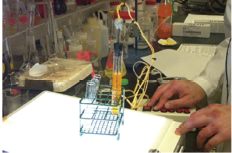
\includegraphics[width=1\linewidth]{fig1.png}
    \caption{Monitoring a color change in a chemical reaction using the SALS and a light box.}
\end{figure}

The SALS control box can also be fitted with a simple conductivity probe that allows it to detect the conductivity difference between two solutions, for example, aqueous and non-aqueous layers in a separatory funnel. This allows the student conducting an organic chemistry experiment to use the separatory funnel, detecting the point at which the more dense solution has passed completely through the stopcock at the bottom. Figure 2 shows the conductivity probe attached to a 25 mL volumetric pipette, which can be immersed into the separatory funnel. This apparatus was developed for a biodiesel synthesis/separation experiment, which was performed by 20 high school students at the National Federation of the Blind (NFB) Youth Slam in summer 2007.

\begin{figure}[!h]
    \centering
    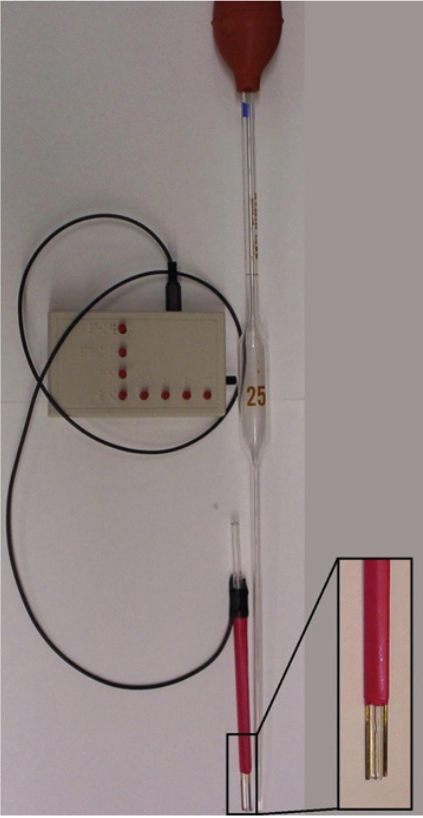
\includegraphics[width=1\linewidth]{fig2.jpeg}
    \caption{A simple ionic conductivity probe (consisting of two insulated wires, exposed at the tip with a gap between them) can be used with the SALS controller box to convert conductivity to audible pitch.}
\end{figure}

\subsection*{Vernier Laboratory Probes and JAWS Scripts}

A number of experiments have been adapted for students who are BLV, using the Vernier Software \& Technology laboratory probe line in conjunction with their Logger Pro 3.5 data collection software package. These have been successfully interfaced with the Job Access with Speech (JAWS) text-to-speech screen reader package by means of the JAWS scripting language, which is flexible enough to allow computer programmers to customize JAWS for applications not envisioned by JAWS software engineers. For the first time, this allows a screen reader to relate all data displayed on Logger Pro. The Vernier probes and JAWS software may be used in conjunction with more recent versions of Logger Pro as well. Additionally, the Ohaus Scout Pro line of balances is among the few types of balances that are Vernier Logger Pro compatible. 

A set of hotkeys allows students who are BLV to listen to real-time probe readings from Logger Pro. The control+shift+S keystroke announces the order of the probes displayed on the sensor line, and corresponding realtime probe readings are announced by using keystrokes constructed in a similar manner: control+shift+1 announces the first probe readings, control+shift+2 announces the second probe readings, etc. If control+shift+S announces temperature, pH, and conductivity, in that order, then control+shift+3 announces readings for the conductivity probe (9). 

Another hotkey is control+shift+A, which announces all objects on the screen. This includes descriptions of X-Y Cartesian graphs, real-time probe readings (both digital and analog), and access to the data table. All are accessible with the control+tab keystroke. When the table is selected, the up, down, left, and right arrows navigate columns and rows of the data table, which are read along with the data displayed at that data point (9). 

Logger Pro also allows the space bar to start and stop data collection, which gives a student who is BLV unprecedented control over data collection. Once collection has concluded, data can be exported into Microsoft Excel, allowing a student who is blind to eliminate bad data points and construct a best-fit line.

Vernier’s Lab Pro serves as a probe interface hub and is connected to a PC via a USB standard cable. The Lab Pro can be powered either by four AA batteries or by AC power. This device contains four analog ports for the Vernier analog probes, as well as two digital sonic ports allowing the use of digital probes such as the Vernier drop counter. The Vernier temperature probe, pH probe, colorimeter, and Vernier drop counter were used in the various experiments in this training workshop. 

Laboratory tools for students with BLV were developed in the 1970s at the Lawrence Hall of Science at UC-Berkeley. Their curriculum, Science Activities for the Visually Impaired/Science Enrichment for Learners with Physical Handicaps (SAVI/SELPH) (10, 11), consists of low- tech (and inexpensive) ways for BLV students to work with non-volatile chemicals; specifically, liquid measurement using notched syringes, Braille-labeled floaters for use in conjunction with graduated cylinders, nontraditional metal thermometers that allow for Braille labels, and easy bench-top organizational methods are stressed. One technique is the utilization of a standard cafeteria tray to be used in the work space of the student who is BLV. All glassware needed for the experiment can be placed on the serving tray by the teacher in advance of the lab period starting. This helps students who are BLV to know exactly where glassware and other essential equipment are located and minimize possible accidents. It also doubles as a spill tray to minimize chemical spills in the work space. 

\section*{OVERVIEW}

On March 1, 2008, the Independent Laboratory Access for the Blind (ILAB) project sponsored a teacher training workshop at the Pennsylvania State University main campus, the purpose of which was to provide a handson laboratory experience both for students who are BLV and teachers from the State College, Pennsylvania, community. This workshop was made eligible for Pennsylvania Act 48 continuing education credit. The workshop was designed to be completed in two hours. A presentation titled “What to Do if a Blind Student Should Enroll in My Science Class,” was presented by Cary Supalo. This presentation discussed various tools for making reading and writing available to the blind, and discussed aspects of legislation and basic teaching techniques and resources available to educators of the blind. A second presentation titled “LowCost Tools and Techniques,” was presented by Thomas Mallouk, which covered some lowcost tool ideas developed by members of the ILAB team, and included techniques developed as part of the SAVI/SELPH curriculum from the Lawrence Hall of Science.

\subsection*{Experiments}

\subsubsection*{Activity 1 (12):}

\textit{Determine Concentrations Using the Colorimeter}

In this experiment, the Vernier colorimeter is used to record the transmittance and absorbance of solutions of water and food dye. Different concentrations of food dye are measured in the colorimeter to determine the percentage of transmittance and amount of absorbance. The colorimeter is an analog probe device that connects to the Vernier Lab Pro by using one of the four analog ports. It emits light from a LED light source through a vial of sample that is then recorded by the Logger Pro data collection software. \textit{Transmittance} is a measurement of the quantity of light that passes through a sample

\[T = \frac{I}{I_{0}}\]

Above is the formula for transmittance, where I\textsubscript{0} is the intensity of the incident light and I is the intensity of the light coming out of the sample. The amount of transmittance recorded from the colorimeter is a percentage. Absorption is the process of absorbing light, while absorbance is the quantity of light being absorbed. Absorbance is relative to the percent of transmittance. The relationship is shown in the equation below. Absorbance is directly related to concentration; the larger the absorbance is, the more concentrated a solution is. 

\[A = log(1/T)\]

\textbf{Materials:}
\begin{itemize}
    \item  3 50 mL beakers
    \item  75 mL water
    \item  1 1 mL syringe
    \item  1 bottle of food dye (green)
    \item  1 glass stirrer
    \item  3 colorimeter cuvettes
    \item  1 colorimeter
    \item  1 Lab Pro
\end{itemize}

Prepare water and food dye solution by adding 25 mL of water in each beaker. Mix in 2, 4 and 6 drops of food dye in the separate  beakers. The beakers should be labeled for the instructor, unknown to students. Buttons on the colorimeter should be Braille-labeled. The colorimeter should be connected to the Lab Pro by means of one of the analog ports, which is then connected to the computer via a USB port. 

Logger Pro 3.5 should be opened at the beginning of the experiment.

\textbf{{Procedure: }}
\begin{enumerate}
    \item The colorimeter should be calibrated before performing the experiment. Check to make sure the wavelength setting on the colorimeter is at 470nm. Fill a cuvette with distilled water.
    \item  Cap the cuvette and place it in the port in the colorimeter. The colorimeter reading is obtained by pressing the space bar on the keyboard. JAWS will announce, “Collection in progress.” After about 10 seconds, press the space bar again to stop the reading and JAWS will announce, “Stop collecting.” There’s a table on the left side of the screen that shows the time in seconds, the percentage of transmittance and the absorption level. At 10 seconds, the transmittance and absorbance is most accurate so the value should be recorded. There should be
100\% transmittance and 0 absorbance.
    \item  Press the CAL button and hold it down for 5 seconds. The absorbance is now calibrated to read 0.000 or 0.001.
    \item  Use the 1 mL notched syringe to draw out solution from the beaker and transfer it into the colorimeter cuvette. Repeat this process so that 2 mL of this food dye solution is in the cuvette.
    \item  Run the colorimeter again by filling the cuvette with the unknown solutions. Record the amount of absorbance. Since absorbance correlates with the concentration of a solution, we can sort the beakers in order of concentration
\end{enumerate}

\subsubsection*{Activity 2 (13):}

\textit{Separation of Aqueous and Organic Layers}

Aqueous and organic liquids will naturally form two layers when put together in a container. This happens because of the “like dissolves like” principle. Polar aqueous liquids will not mix with non-polar organic liquids. One method to separate these two layers is with a separatory funnel. In this experiment a separatory funnel and the Submersible Audible Light Sensor (SALS) are used to separate water and vegetable oil.

\newpage
\textbf{Materials:}

\begin{itemize}
    \item  1 250 mL separatory funnel
    \item  1 100 mL graduated cylinder
    \item  1 50 mL graduated cylinder
    \item  1 25 mL plastic syringe
    \item  100 mL water
    \item  50 mL vegetable oil
    \item  1 100 mL beaker
    \item  2 250 mL beakers
    \item  1 ring stand
    \item  1 funnel
    \item  1 400 mL beaker
    \item  1 1000 mL beaker
    \item  1 SALS sensor and conductivity probe
\end{itemize}

\textbf{Procedure:}

\begin{enumerate}
    \item Measure out 100 mL of water into the 100 mL graduated cylinder using a 25 mL notched syringe. Keep the 100 mL graduated cylinder in one of the 500 mL beakers while measuring to minimize spillage. Pour the water into the 250 mL separatory funnel using the funnel. Make sure the stopcock is closed when pouring liquid into it.
    \item Measure out 50 mL of vegetable oil into the 50 mL graduated cylinder using a 25 mL notched syringe. Keep the 50 mL graduated cylinder in one of the 500 mL beakers while measuring to minimize spillage. Pour vegetable oil into the 250 mL separatory funnel using the funnel.
    \item At this point the SALS sensor will be used to distinguish between the two layers of liquid. Turn on the SALS sensor by holding the Power button (the top button on the left of the SALS sensor) for two seconds. Press the Play button (the second button, underneath Power) until the SALS sensor says “Constant Tone Mode.” After this, mo the conductivity probe up and down in  liquid to hear a tone difference between  oil layer and the water layer.
    \item Lower the conductivity probe to rest at the bottom of the separatory funnel.
    \item Open the stopcock on the separatory funnel so that the water layer begins to drain out of the separatory funnel and into the 250 mL beaker. When the tone changes, close the stopcock and the two layers will have been separated. The oil layer should completely remain in the separatory funnel; the water layer will have been separated out.
    \item Dispose of the materials in the appropriate waste container
\end{enumerate}

\subsubsection*{Activity 3 (14):}

\textit{Blue Bottle Reaction}

The “Blue Bottle Reaction” is a great way to demonstrate the change in color of a solution due to the effects of oxidation. The solution will start out blue and gradually become colorless. The blue color can be restored if the solution is shaken up again. The use of the SALS sensor in this experiment will prove to be very helpful in detecting those color changes.

\textbf{Materials:}

\begin{itemize}
    \item  Tap water
    \item  One 1 L Erlenmeyer flask, with stopper
    \item  2.5 grams glucose
    \item  2.5 grams sodium hydroxide
    \item  0.1\% solution of methylene blue
\end{itemize}

\textbf{Procedure:}
\begin{enumerate}
    \item 1. Fill the Erlenmeyer flask half full with tap water by using a SAVI/SELPH volumetric floater device.
    \item Measure 2.5 grams of glucose on the Ohaus Scout Pro balance by using the JAWS with Logger Pro interface. Dissolve the glucose in the water.
    \item Measure and dissolve the 2.5 grams of sodium hydroxide in the flask.
    \item Use notched syringe to add 1 mL of 0.1\% methylene blue to the flask.
    \item Put the stopper on the flask and shake to dissolve the dye. The solution at this time should be blue.
    \item To determine the change in color, use the SALS sensor. Turn it on by pressing and holding the Power button. In order to hear the tone continuously so that the change in color will be easier to detect, hold the Play button down until you hear the sensor speak “Constant Tone Mode.”
    \item Remove the stopper and insert the SALS sensor probe into the solution in the flask.
    \item The color of the solution will slowly change from blue to clear as the methylene blue is oxidized from the air.
    \item To see the blue color again, swirl the solution in the flask. The solution will change from clear to blue and back to clear.
    \item When finished, the contents of the reaction can be poured down the drain with excess water
\end{enumerate}

\section*{SUMMARY}

These experiments illustrate how ILAB tools can be incorporated into a teacher training module to introduce educators to the tool functionality. These experiments can be expanded to include other aspects of science. Additional Vernier Software \& Technology products can be incorporated into other science activities to further demonstrate how ILAB tools can assist educators when working with students who are BLV. The curriculum published by Vernier Software \& Technology can also be used in similar workshops to further illustrate the JAWS with Logger Pro interface. For more information about adaptations, go to \url{http://ilab.psu.edu}.

These workshops can be made eligible for continuing education credits based on individual state requirements. Workshops similar to this one can serve as educational venues for current and future educators to serve students who are BLV. These tools do require some level of training both for teachers and the students. The more practice in advance of a class starting, the better the experience both the teacher and the BLV student will have with the tools, thus enhancing their learning experience

\end{large}
\clearpage
\section*{REFERENCES}\par 

\leftskip 0.25in
\parindent -0.25in 

DeLaGarza, D.V. \& Erin, J.N. (1993). Employment Status and Quality of Life of Graduates of a State Residential School. Journal of Visual Impairment and Blindness, 87 (6), 229-233.

De Luchi, L., Malone, L. (1982). SAVI (Science Activities for the Visually Impaired). In Mangold, S. (Ed.), A teacher’s guide to the special educational needs of blind and visually handicapped children (pp. 72-93). American Foundation for the Blind: New York, NY. 

Helmenstine, A M. How to Do the Blue Bottle Chemistry Demonstration. \url{http://chemistry.about.com/od/chemistrydemonstrations/ss/bluebottle.htm} (accessed August 2009).

Holmquist, D.D. \& Volz, D.L. (2003). Chemistry with Computers: Chemistry Experiments Using Vernier Sensors (pp. 11-1 – 11-2T). Vernier Software \& Technology: Beaverton, OR. 

Matson, F. (1990). Walking Alone and Marching Together (p. 375). National Federation of the Blind: Baltimore, MD.

McCartney, B.D. (1993). Challenges Facing Residential Schools: A Case Study. Journal of Visual Impairment and Blindness, 87 (6), 204-5.

Miner, D., Nieman, R., Swanson, A.B., Woods, M., Eds. (2001). Teaching Chemistry to Students with Disabilities: A Manual for High Schools, Colleges, and Graduate Programs, 4th ed. (pp. 4, 10). American Chemical Society: Washington, DC.

Omvig, J.H. (2002). Freedom for the Blind: The Secret Is Empowerment. University of Arkansas Press: Fayetteville, AR. Day, Richard (1995). Habilitate – Then Educate. Re:view, XXVII (2), 83-86.

Scadden, L. (2005). Current status of people with disabilities in STEM education: a personal perspective. Paper presented at RASEMSquared, October 2005.

Science Activities for the Visually Impaired/Science Enrichment for Learners with Physical Handicaps (SAVI/SELPH) Web site, \url{http://www.lawrencehallofscience.org/cml/saviselph.html} (accessed August 2009).

Supalo, C., Mallouk, T., Amorosi, C., Rankel, L.A., Wohlers, H.D., Roth, A., Greenberg, A. (2007). Talking Tools to Assist Students Who Are Blind in Laboratory Courses. Journal of Science Education for Students with Disabilities, 12 (1), 27-32.

Supalo, C., Mallouk, T., Musser, A., Han, J., Briody, E., McArtor, C., Gregory, K., Kreuter, R. (2006). Seeing Chemistry through Sound: A Submersible Audible Light Sensor for Observing Reactions in Real Time. Assistive Technology Outcomes and Benefits, 3 (1), 110-116.

Supalo, C.A., Mallouk, T. E., Amorosi, C., Lanouette, J., Wohlers, H.D., McEnnis, K. (2009). Using Adaptive Tools and Techniques to Teach a Class of Students Who Are Blind or Low Vision. Journal of Chemical Education, 86 (5), 587-591

\end{document}
